\subsection{Introducción}

En esta sección se buscó implementar la siguiente máquina de estados finitos:
\begin{figure}[H]
\centering
	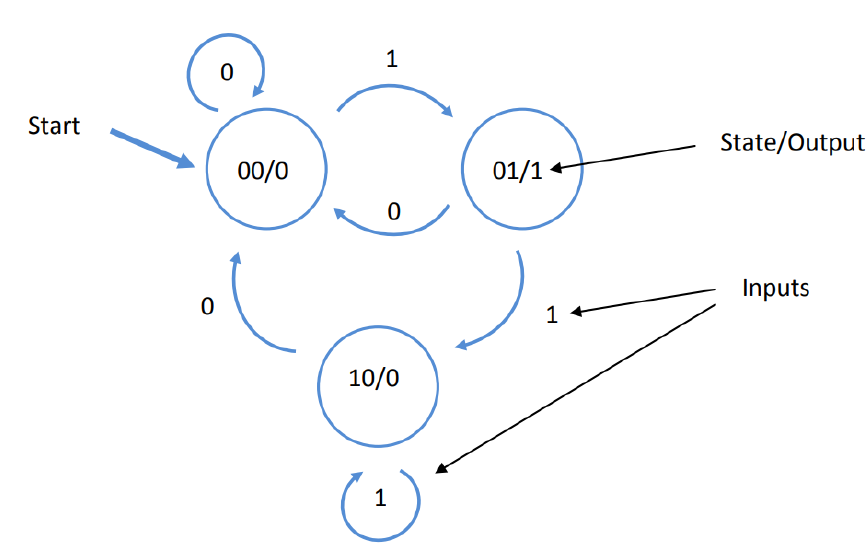
\includegraphics[width=0.6\textwidth]{ImagenesEjercicio3/fsm.png}
	\caption{Máquina de estados finitos a implementar.}
	\label{fig:fsmimp}
\end{figure} 

Para esto, se conformó la tabla de estados considerando al estado $00$ como el inicial, resultando:
\begin{table}[H]
\centering
\begin{tabular}{|c|l|c|l|c|l|c|}
\hline
\multicolumn{2}{|c|}{\multirow{2}{*}{$Present State$}} & \multicolumn{4}{c|}{$Next State$} & \multirow{3}{*}{$Output (z)$} \\ \cline{3-6}
\multicolumn{2}{|c|}{} & \multicolumn{2}{c|}{$w=0$} & \multicolumn{2}{c|}{$w=1$} &  \\
\multicolumn{2}{|c|}{$y_2 y_1$} & \multicolumn{2}{c|}{$Y_2Y_1$} & \multicolumn{2}{c|}{$Y_2Y_1$} &  \\ \hline
\multicolumn{2}{|c|}{00} & \multicolumn{2}{c|}{00} & \multicolumn{2}{c|}{01} & 0 \\ \hline
\multicolumn{2}{|c|}{01} & \multicolumn{2}{c|}{00} & \multicolumn{2}{c|}{10} & 1 \\ \hline
\multicolumn{2}{|c|}{10} & \multicolumn{2}{c|}{00} & \multicolumn{2}{c|}{10} & 0 \\ \hline
\multicolumn{2}{|c|}{11} & \multicolumn{2}{c|}{xx} & \multicolumn{2}{c|}{xx} & x \\ \hline
\end{tabular}
\caption{Tabla de estados para la máquina de estados finita a implementar.}
\label{fig:tablaestados}
\end{table}

Como fue necesario implementar tres estados, se requirió utilizar dos flip-flops. Luego, se hallaron las fórmulas lógicas para los estados siguientes utilizando mapas de Karnaugh.
\begin{figure}[H]
\begin{subfigure}{0.49\textwidth}
\begin{centering}
    \begin{Karnaughvuit}
        \minterms{5, 6}
        \maxterms{0,1,2,4}
        \indeterminats{7, 3}
        
        \implicant{5}{7}{orange}
        \implicant{7}{6}{blue}
        
    \end{Karnaughvuit}
\par\end{centering}

\begin{equation*}
Y_2 = wy_1+wy_2
\end{equation*}
\begin{table}[H]
\caption{Solución para $Y_2.$}
\label{mapa:Y2}
\end{table}
\end{subfigure}
\begin{subfigure}{0.49\textwidth}
\begin{centering}
    \begin{Karnaughvuit}
        \minterms{4}
        \maxterms{0,1,2,5,6}
        \indeterminats{7,3}
        
        \implicantsol{4}{green}
        
    \end{Karnaughvuit}
\par\end{centering}
\begin{equation*}
Y_1 = w(\overline{y_2}\cdot \overline{y_1})
\end{equation*}
\begin{table}[H]
\caption{Solución para $Y_1.$}
\label{mapa:Y1}
\end{table}
\end{subfigure}
\caption{Mapas de Karnaugh para los próximos estados de la maquina de estados finitos.}
\end{figure}

Utilizando el teorema de De Morgan y simplificando se obtienen dos posibles implementaciones análogas:
\begin{figure}[H]
\begin{subfigure}{0.49\textwidth}
\vspace*{-0.17cm}
\begin{equation*}
\left\{
\begin{aligned}
		& Y_1 = w(\overline{y_2}\cdot \overline{y_1})	 \\		
		& Y_2 = w\overline{(\overline{y_2}\cdot \overline{y_1})}\\		
\end{aligned}
\right.
\end{equation*}
\caption{Implementación con NAND.}
\end{subfigure}
\begin{subfigure}{0.49\textwidth}
\begin{equation*}
\left\{
\begin{aligned}
		& Y_1 = w(\overline{y_2+y_1}) \\		
		& Y_2 = w(y_2+y_1)\\		
\end{aligned}
\right.
\end{equation*}
\caption{Implementación con AND y NOR.}
\end{subfigure}
\end{figure}

Si este circuito fuese trabajado directamente sobre el silicio, se elegiría la implementación con compuertas NAND, ya que esta forma es la más simple de realizar. Sin embargo, como se realizó sobre un PCB, se decidió utilizar la implementación con AND y NOR, debido a que de esta manera se utilizan solamente dos integrados para el circuito lógico de entrada y salida, a diferencia de la implementación con NAND, el cual requiere de tres integrados, utilizando un total de nueve NAND's. Finalmente, a partir de las ecuaciones obtenidas se esquematizó la implementación teórica.

\begin{figure}[H]
	\centering
	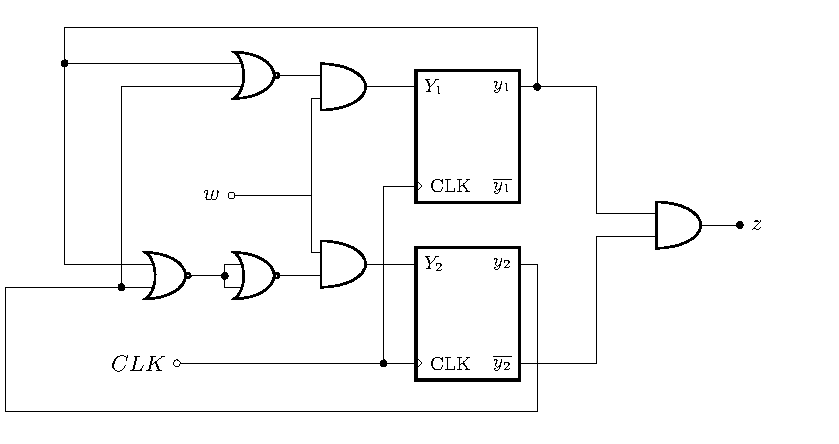
\includegraphics[width=0.8\textwidth, page=1]{ImagenesEjercicio3/Maquina.pdf}
	\caption{Implementación teórica de la lógica de entrada, estados y lógica de salida.}
\end{figure}


\subsection{Simulación}

Se simuló la implementación obtenida en la sección anterior utilizando $Verilog$. Además, se construyó un test bench con todas las combinaciones posibles de entradas. Esta simulación obtuvo resultados exitosos. Se encuentra anexada esta simulación junto al test bench y un ejecutable junto a este informe.

\subsection{Implementación}
Para esta etapa se tuvo un cuidado especial dado que era un requisito en la implementación que la lógica interna del circuito funcione con $3.3 \ V$, mientras que las entradas y salidas debían operar con $5 \ V$.

\subsubsection{Level Shifting}
Para la conversión de $3.3 \ V$ a $5 \ V$ de la salida se decidió utilizar un transistor bipolar NPN como indica la Figura (\ref{circ:stepup}). Luego, para las entradas, las cuales deben pasar de $5 \ V$ a $3.3 \ V	$, se utilizó un diodo zener de $3.3 \ V$ con una resistencia limitadora de corriente, la cual fue calculada conociendo la corriente de codo del diodo y la corriente de entrada de las compuertas de tecnología CMOS empleadas. Esta implementación se puede observar en la Figura(\ref{circ:stepdown}). 

\begin{figure}[H]

	\centering
	\begin{subfigure}{0.49\textwidth}
		\centering
		\begin{circuitikz}
			\draw
			(0,0)
			node[ocirc, label=west:$In$](in){}
			++(2, 0) node[npn, rotate=-90](npn){}
			(npn.B) ++ (0, 2)node[ocirc, label=north:$3.3 \ V$](3v3){}
			(3v3)to[R=$2.2 \ k\Omega$]++(0, -2)
			(3v3)++(2, 0)node[ocirc, label=north:$5 \ V$](5v){}
			(5v)to[R=$6.8 \ k\Omega$]++(0, -2)to[short, -*]++(0, -0.83)
			(npn.C) to[short]++(2.5, 0)node[ocirc, label=east:$Out$]{}
			(npn.E)--(in.center)			
			;
		\end{circuitikz}
		\caption{\centering Transistor NPN en base común utilizado como step-up level-shifter.}
		\label{circ:stepup}
	\end{subfigure}
	\begin{subfigure}{0.49\textwidth}
	\centering
	\begin{circuitikz}
			\draw
				(0,0)
				node[ocirc, label=west:$In$]{}
				to[R, l^=$100 \ \Omega$]++(2.5,0)
				to[open]++(0, -2)
				node[tlground]{}
				to[full ZZener diode, l_=$3.3 \ V$, -*] ++ (0, 2)
				
				to[short] ++ (1, 0)
				node[ocirc, label=east:$Out$]{}
				%%%%%%%%%%%%%%%%%%%%%%%%%%
				to[open]++(0, 1.45)
			;
		\end{circuitikz}
		\caption{\centering Regulador de tensión de $3.3 \ V$ con zener y resistencia utilizados como step-down level-shifter.}
		\label{circ:stepdown}
	\end{subfigure}

\end{figure}

\subsubsection{Diseño Final}

Finalmente se presenta a continuación el diseño final de la máquina de estados finitos implementada en un PCB de $50 mm \ x \ 50 mm$.

\begin{figure}[H]
	\centering
	\includegraphics[width=\textwidth, page=2]{ImagenesEjercicio3/Maquina.pdf}
	\caption{Implementación de la máquina de estados finitos junto a la conversión de niveles de tensión.}
\end{figure}
	
\subsubsection{Componentes}
A continuación se detallan los componentes utilizados en la implementación:
\begin{itemize}
\item Dual Flip-flop D: \href{http://www.ti.com/lit/ds/symlink/cd4013b.pdf}{CD4013}
\item Quad 2-input AND: \href{https://www.mouser.com/datasheet/2/308/74HC08.REV1-102589.pdf}{74HC08}
\item Quad 2-input NOR: \href{https://assets.nexperia.com/documents/data-sheet/74HC_HCT02.pdf}{74HC02}
\item BJT NPN: \href{http://www.philohome.com/sensors/gp2d12/gp2d12-datasheets/bc548.pdf}{BC548}
\end{itemize}

\subsection{Mediciones}

Se realizaron mediciones de tanto correcta transición entre estados como de niveles de tensión en el circuito.

\begin{figure}[H]
\begin{subfigure}{0.49\textwidth}
\centering
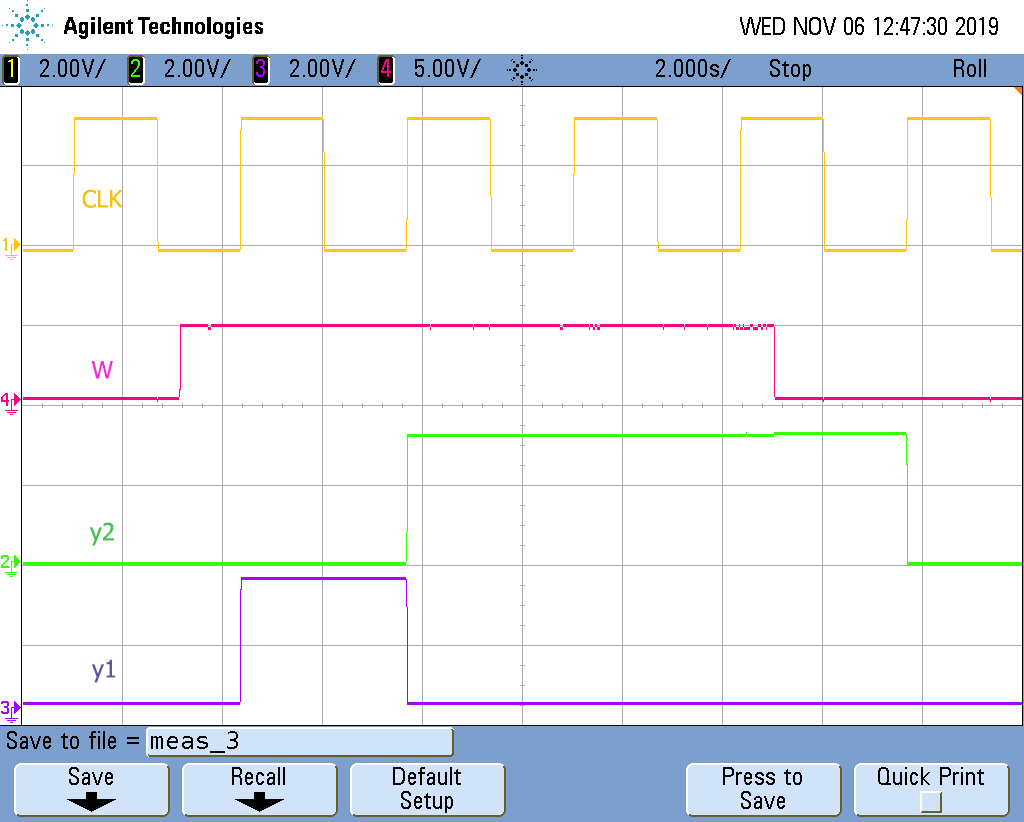
\includegraphics[width=\textwidth,trim={0 3.35cm 0.1cm 1.75cm},clip]{ImagenesEjercicio3/states.png}
\caption{Medición de transiciones de estados: ..00-01-10-...-10-00-..}
\label{states1}
\end{subfigure}
\begin{subfigure}{0.49\textwidth}
\centering
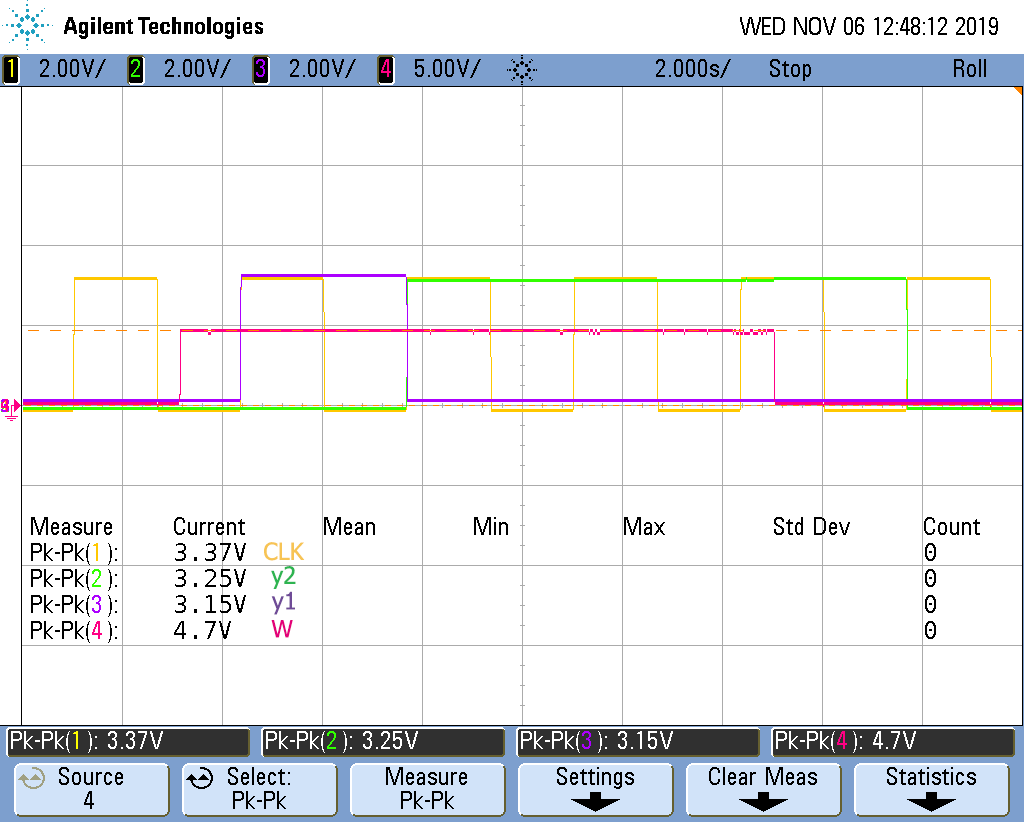
\includegraphics[width=\textwidth,trim={0 3.35cm 0.1cm 1.75cm},clip]{ImagenesEjercicio3/vlevels_states.png}
\caption{Medición de los niveles de tensión.}
\end{subfigure}
\caption{Mediciones del circuito implementado.}
\end{figure}

\begin{figure}[H]
\centering
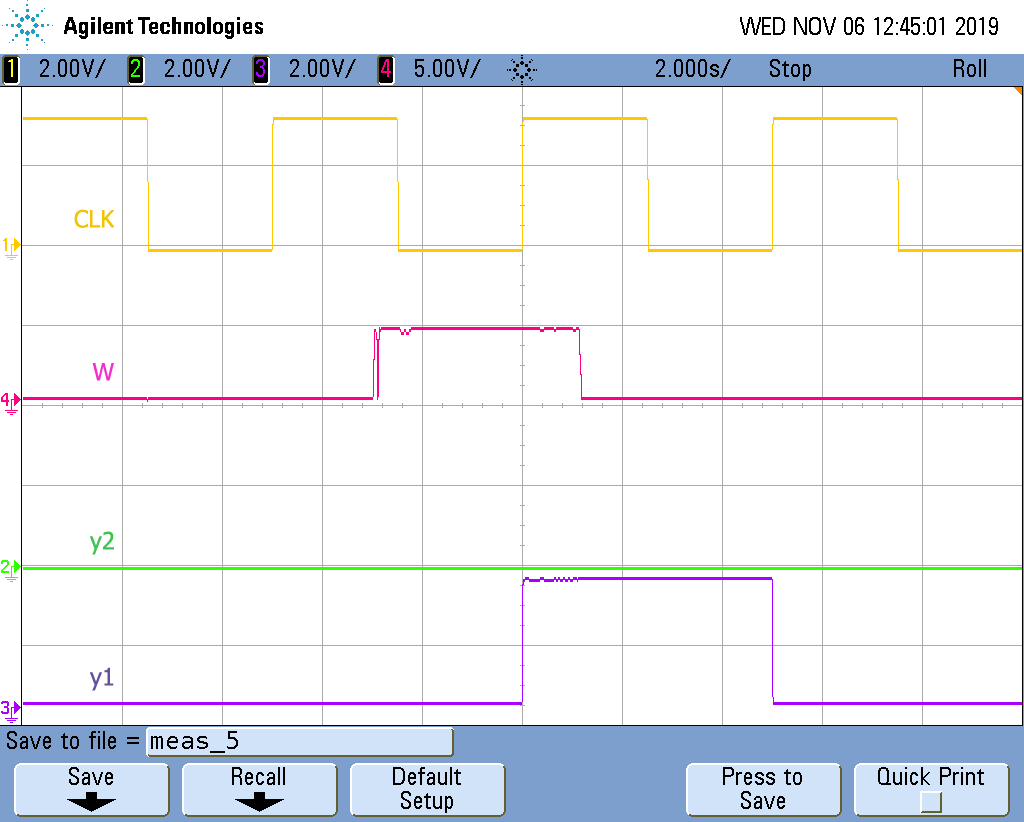
\includegraphics[width=0.7\textwidth,trim={0 3.35cm 0.1cm 1.75cm},clip]{ImagenesEjercicio3/states2.png}
\caption{Medición de la transición de estados: ..00-01-00-..}
\label{states2}
\end{figure}

\begin{figure}[H]
\begin{subfigure}{0.49\textwidth}
\centering
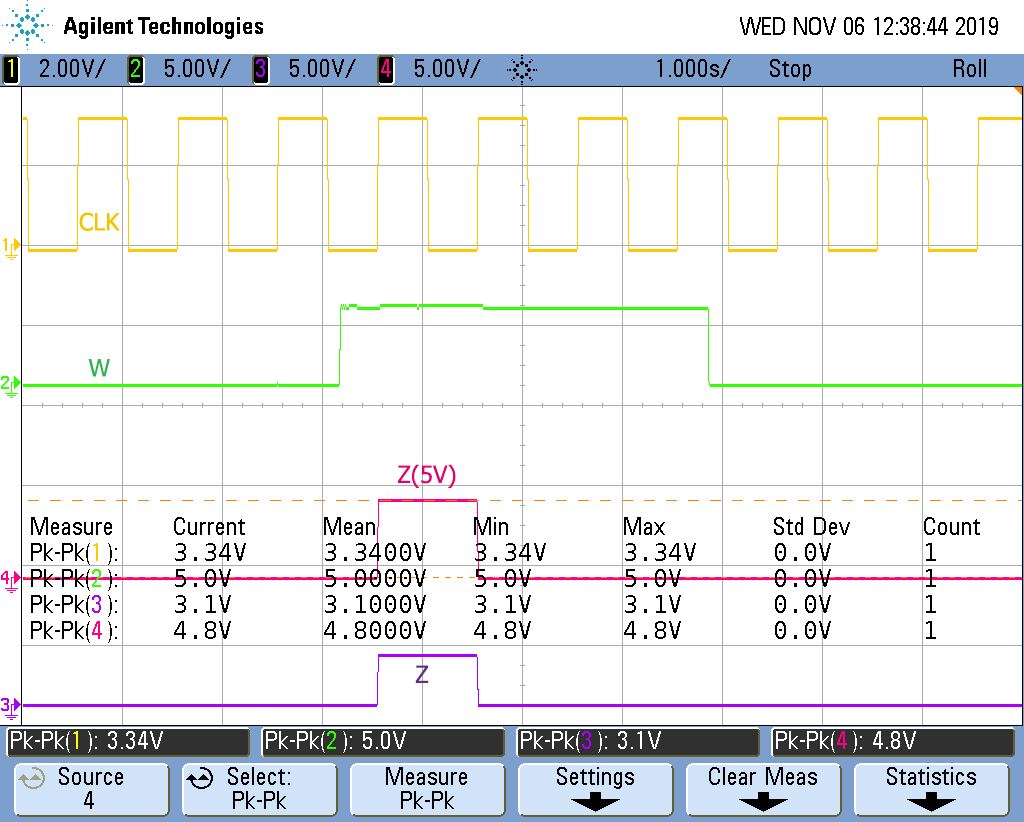
\includegraphics[width=\textwidth,trim={0 3.35cm 0.1cm 1.75cm},clip]{ImagenesEjercicio3/output.png}
\caption{Medición de la transición de la salida del circuito.}
\label{output}
\end{subfigure}
\begin{subfigure}{0.49\textwidth}
\centering
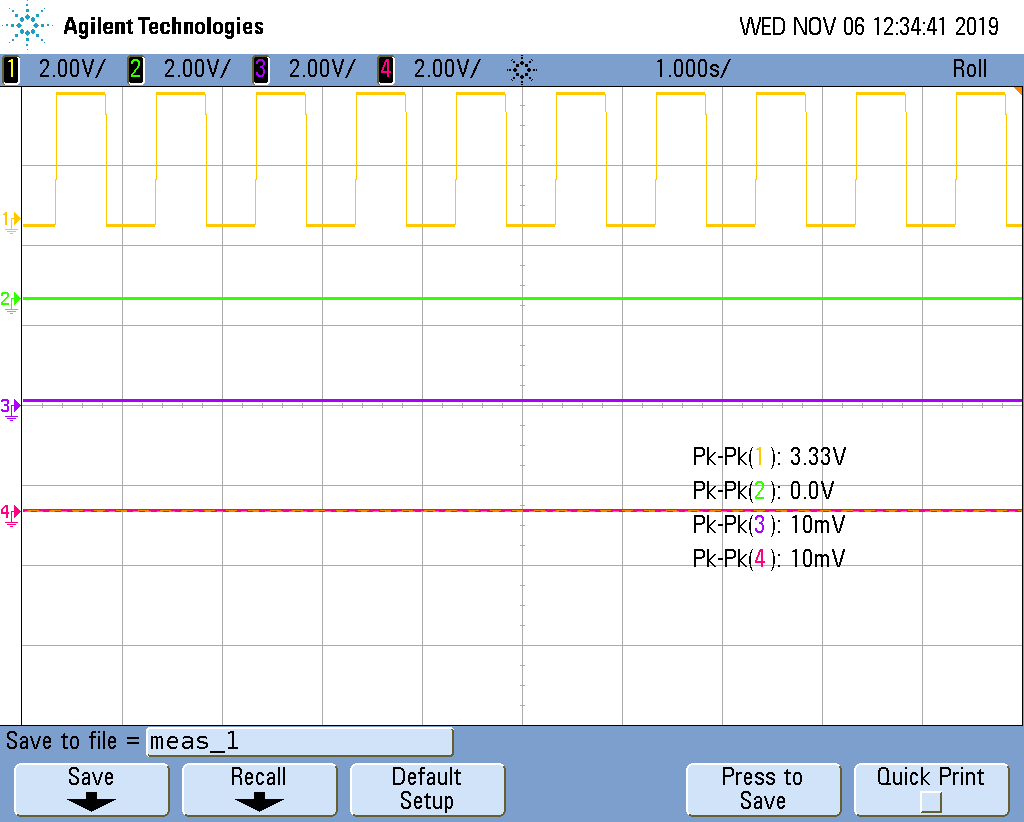
\includegraphics[width=\textwidth,trim={0 3.35cm 0.1cm 1.75cm},clip]{ImagenesEjercicio3/vlevels_low.png}
\caption{Medición de los niveles de tensión en estado bajo..}
\end{subfigure}
\caption{Mediciones del circuito implementado.}
\end{figure}

Se puede observar que el level shifting de niveles de tensión funcionan correctamente. Los niveles de tensión son:
\begin{itemize}
\item $V_{OL} = 10 \ mV$
\item $V_{OH} = 4.8 \ V$
\item $V_{3.3_{H}} \geq 3.1 \ V$
\item $V_{3.3_{L}} \approx 0 \ V$
\end{itemize}

Se destaca que $V_{3.3}$ representa el nivel de tensión de la lógica interna del circuito, mientras que $V_{OL}$ y $V_{OH}$ son los niveles de tensión altos y bajos conseguidos a la salida $Z$.

Luego, se observa en las Figuras (\ref{states1}) y (\ref{states2}) que la transición de estados funciona correctamente habiendo probado todas las combinaciones posibles. Por otro lado, en la Figura (\ref{output}) se observa que la salida posee los valores adecuados, siendo cero para todos los estados excepto en el $01$, para el cual la salida es igual a un uno lógico. Finalmente, se destaca que el consumo de corriente del circuito es de $15 \ mA$ en todos los estados excepto en el estado $01$ posee un consumo de $32 \ mA$.

\subsection{Conclusiones}

Se implementó la FSM propuesta habiendo cumplido los requisitos de niveles de tensión de lógica interna. Si bien la transición de $5 \ V$ a $3.3 \ V$ funcionó correctamente, el consumo de corriente es muy elevado, observandose un máximo de $32 \ mA$. Si se hubiera deseado un consumo menor, se debería utilizar un step-down level-shifters, valiéndose transistores como se realizó para el step-up level-shifter. Este logró mantener la salida en una tensión muy baja para el estado lógico bajo y en una tensión aceptable para el estado de tensión lógico alto, con un error de $200 \ mV$ por debajo del deseado. Sin embargo, estos niveles de tensión se encuentran totalmente dentro de estándares de márgenes de ruido tanto para la tecnología TTL como para CMOS. Luego, la tensión alta de la lógica interna de $3.1 \ V$ se encuentra también dentro de los márgenes de ruido para ambas tecnologías.

Otras posibles implementaciones para el step-down parten del uso de un divisor resistivo, lo cual disminuye el consumo de corriente, ya que dentro de los valores de resistencias que se pueden utilizar, se hayan aquellas de $10 \ k\Omega$ o más, ya que estos valores no son lo suficientemente altos como para generar un divisor resistivo con la impedancia de entrada de la compuerta CMOS ni para provocar una corriente comparable con el consumo de estas compuertas. Otra implementación se centra en el uso de un comparador. Este último es más barato que un transistor, pero se descartó por su gran tamaño y por poseer implementaciones más simples con mismo resultado.